\begin{frame}
\frametitle{Obbiettivi del Progetto}
\begin{block}{Finalità}
Obbiettivo principale: fornire un ausilio alle
persone il cui compito è la gestione logistica di 
un dipartimento universitario:
\begin{itemize}
\item Gestione del personale afferente al dipartimento
\item Gestione degli spazi dipartimentali
\item Verifica e controllo dell'allocazione degli spazi al personale
\item Inventariazione delle attrezzature a disposizione del dipartimento
\end{itemize}
\end{block}
\end{frame}

\begin{frame}
\frametitle{Realtà di interesse}
\begin{block}{Entità fondamentali}
La realtà in esame è assai complessa $\rightarrow$
creazione di un modello concettuale
che modellizzi la realtà.

Ci si è avvalsi della teoria insiemistica:
\begin{itemize}
\item Insieme delle risorse spaziali SRES
\item Insieme delle risorse umane HRES
\item Insieme delle attrezzature ATTR
\end{itemize}
Gli elementi degli insiemi sono le entità fondamentali
del modello.
\end{block}
\begin{block}{}
La realtà analizzata è un esempio di sistema concorrente
complesso.
\end{block}
\end{frame}


\begin{frame}
\frametitle{Linee guida per lo sviluppo}
\begin{block}{Caratteristiche del software}
\begin{itemize}
\item Deve permettere a diversi utenti di interagire coi dati
\item Divisione dell'utenza in due macrocategorie
\begin{itemize}
\item admin-side
\item user-side
\end{itemize}
\item Efficienza e semplicità di utilizzo
\end{itemize}
\end{block}
\begin{block}{Principi di sviluppo}
\begin{itemize}
\item Portabilità
\item Scalabilità
\item Modularità
\end{itemize}
\end{block}
\end{frame}

\begin{frame}
\frametitle{Web-Application}
\begin{block}{Pro}
Le caratteristiche desiderate sono in accordo con le peculiarità di una web-application:
\begin{itemize}
\item Architettura Server-Client:
\begin{description}
\item [Server] memorizzazione fisica del software e dei dati
\item [Client] accesso alla \emph{webapp} tramite un Web-Browser
\end{description}
\item Possibilità di realizzare un servizio di autenticazione
\item Possibilità di ulteriori sviluppi futuri grazie allo sviluppo del Web
\item Familiarità di qualsiasi utente con una pagina web
\end{itemize}
\end{block}
\begin{block}{Contro}
\begin{itemize}
\item Necessità di disporre di un network per utilizzare l'applicazione
\item Server \emph{down} $\rightarrow$ applicazione inaccessibile ai client
\end{itemize}
\end{block}
\end{frame}

\begin{frame}
\frametitle{Ambiente di Sviluppo}
\begin{block}{LAMP}
Per sviluppare il progetto si è utilizzato l'ambiente
\emph{LAMP} (\emph{Open Source Software})
\begin{description}
\item [L]inux: Debian GNU/Linux 4.1 \emph{sid} release (OS)
\item [A]pache v2.2.6 (Web-Server)
\item [M]ySQL v5.0.5 (RDBMS)
\item [P]HP v5.2.5 (Linguaggio di programmazione)
\end{description}
Nello specifico è stato utilizzato il pacchetto di
sviluppo XAMPP v1.6.5
\end{block}
\begin{block}{}
Il software xAMP è disponibile anche per MacOSX\cpr{} e Windows\cpr{}
\end{block}
\end{frame}

\begin{frame}
\frametitle{Base di Dati}
\begin{columns}[c]
\begin{column}{5.5cm}
\begin{block}{}
Si è utilizzata la teoria relazionale per implementare il
modello concettuale
\end{block}
\begin{block}{Procedura progettuale}

\begin{itemize}
\item realizzazione dello schema ER complessivo della realtà
di interesse, mediante raffinamenti successivi
\item 
creazione dello schema  logico-relazionale 
(vincoli di integrità referenziale e verifica della \emph{BCNF})
\item implementazione in MySQL\cpr{}, mediante linguaggio SQL
\end{itemize}

\end{block}
%\end{frame}
\end{column}

%\begin{frame}
%\frametitle{Schema ER}
\begin{column}{4.5cm}
\begin{figure}[htbp]
\begin{center}
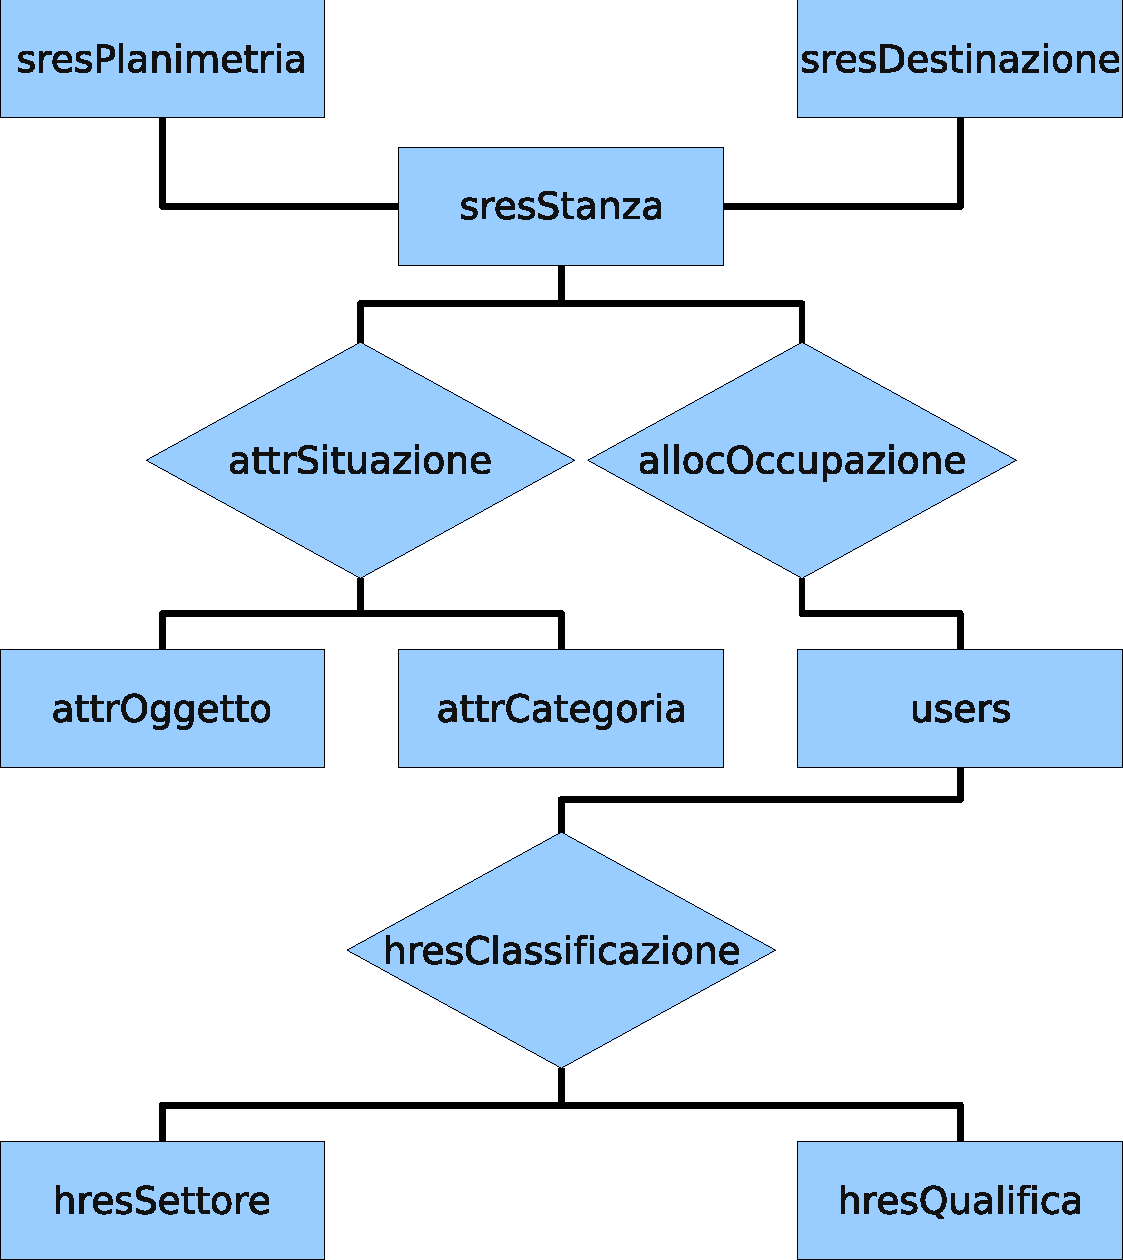
\includegraphics[width=3.5cm]{image/SchemaERcompleto.pdf}
	\caption {Schema ER complessivo}
	\label{schemaER}
\end{center}
\end{figure}
\end{column}
\end{columns}
\end{frame}

%\begin{frame}
%\frametitle{Comunicazione fra processi LAMP}
%\begin{block}{}
%È necessario che il software  possa comunicare con il 
%Web-Server e con il RDBMS:
%\begin{itemize}
%\item Accesso alla base di dati, rappresentazione della realtà
%\item Accesso ai dati conservati dal Web-Server provenienti dal
%Web-Client
%\end{itemize}
%\end{block}
%\begin{block}{}
%\begin{description}
%\item [Web Server] array associativo superglobale \texttt{\$\_REQUEST[]} costituito di coppie \texttt{(variable,value)}
%\item [MySQL] librerie del \emph{core} di PHP\cpr{}$\rightarrow$ realizzazione di una classe (\emph{object-oriented})
%\end{description}
%\end{block}
%\end{frame}

\begin{frame}
\frametitle{Struttura dell'applicazione}
\begin{block}{Struttura a 2 livelli}


\begin{columns}[t]

\begin{column}{5cm}
\begin{itemize}
\item \emph{framework}
\begin{itemize}
\item Login
\item Authentication
\item Page Generation
\end{itemize}
\item \emph{tools}
\begin{itemize}
\item Moduli per realizzare task specifici
\end{itemize}
\end{itemize}
\end{column}

\begin{column}{5cm}
\begin{figure}[htbp]
%\begin{center}
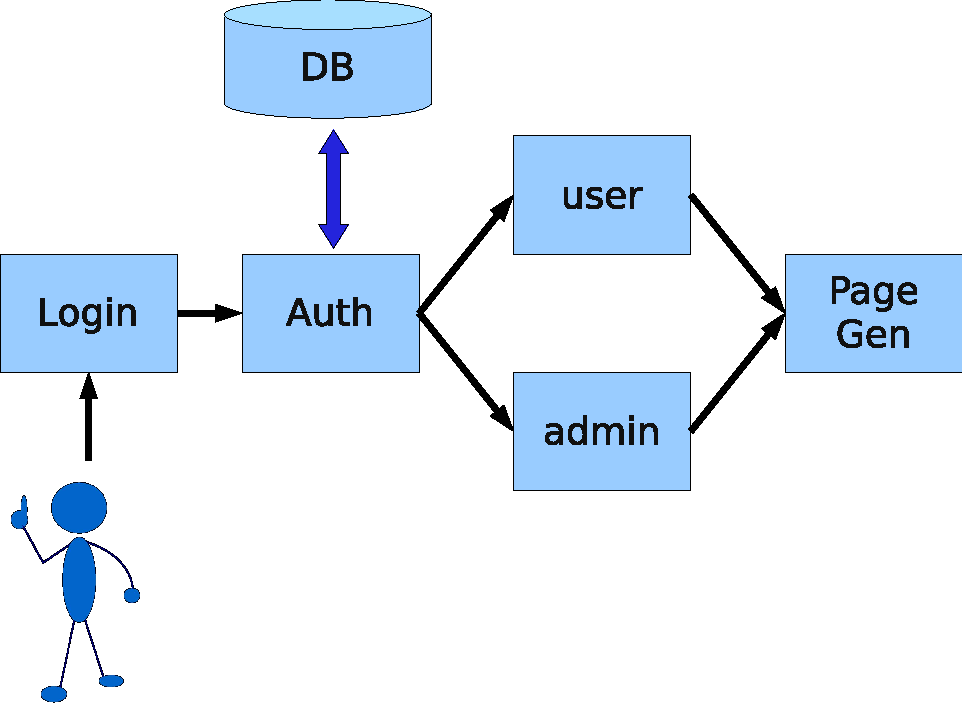
\includegraphics[width=3cm]{image/SchemaAppLogin-PageGen.pdf}
	\caption {Il \emph{framework} della \emph{WebApp}}
	\label{parte1webapp}
%\end{center}
\end{figure}
\end{column}

\end{columns}
\end{block}

\begin{block}{}
\begin{itemize}
\item Il \emph{framework} è lo scheletro dell'applicazione sul quale si innestano i \emph{tools}
\item I \emph{tools} sono script indipendenti dal \emph{framework} che costituiscono il 
corpo della pagina \emph{web} $\rightarrow$ 
modifica del software a questo livello
\end{itemize}
\end{block}

\end{frame}

%\begin{frame}
%\frametitle{Il \emph{framework}}
%\begin{figure}[htbp]
%\begin{center}
%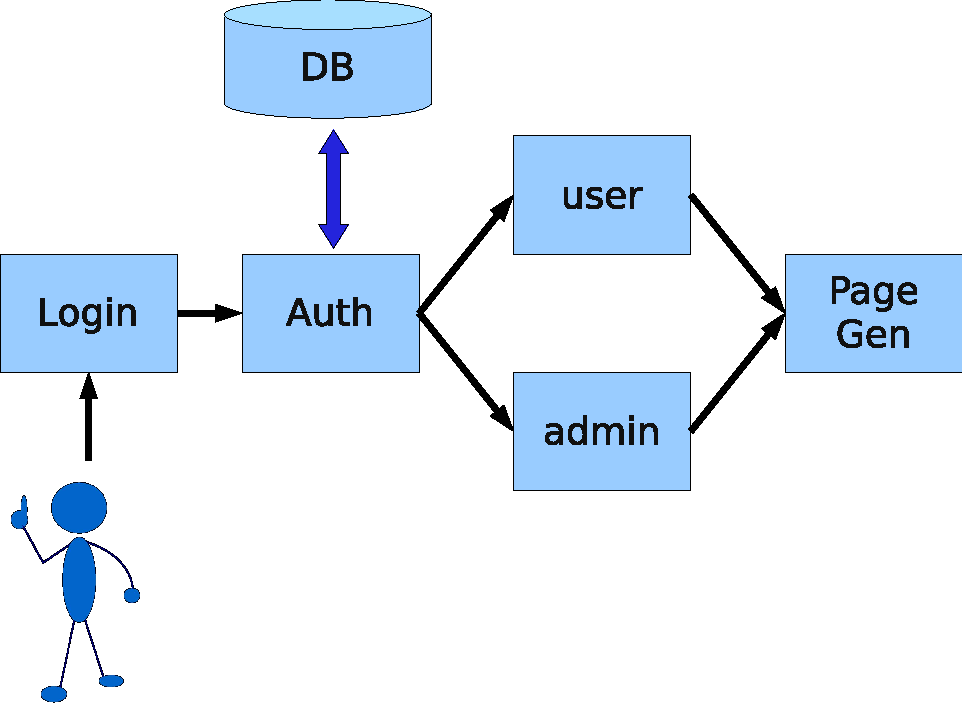
\includegraphics[width=8cm]{image/SchemaAppLogin-PageGen.pdf}
%	\caption {Schema a blocchi rappresentante il \emph{framework} della \emph{web-application}}
%	\label{parte1webapp}
%\end{center}
%\end{figure}
%\end{frame}

\begin{frame}
\frametitle{Tools realizzati - 1}
\begin{block}{}
\begin{description}[Risorse Spaziali]
\item [Risorse Spaziali] provvede alle gestione dell'insieme SRES
\begin{itemize}
\item Planimetrie
\item Locali
\item Destinazione d'uso
\end{itemize}
\item [Risorse Umane] dedicato al controllo dell'insieme HRES
\begin{itemize}
\item Settori di Afferenza
\item Qualifiche Professionali
\end{itemize}
\item [Allocatore] permette l'assegnazione delle risorse spaziali
al personale afferente al dipartimento
\begin{itemize}
\item Visualizzazione Stato
\item Allocazione manuale tabellare
\item Allocazione guidata tabellare
\end{itemize}
\end{description}
\end{block}
\end{frame}


\begin{frame}
\frametitle{Tools realizzati - 2}
\begin{block}{}
\begin{description}[Communicator]
\item [Attrezzature] realizzato per la gestione di ATTR 
\begin{itemize}
\item Oggetti in astratto
\item Oggetti reali (inventario e disponibilità)
\item Categorie
\end{itemize}
\item [Communicator] fornisce agli utenti della \emph{webapp}
un servizio di messaggistica
\begin{itemize}
\item Invio e ricezione messaggi agli utenti della \emph{webapp}
\item Archiviazione messaggi
\item Servizio interno all'applicazione
\end{itemize}
\end{description}
\end{block}
\end{frame}


\begin{frame}

\frametitle{Screenshot della \emph{WebApp}}

\begin{columns}[t]

\begin{column}{6cm}
\begin{figure}[htbp]
%\centering
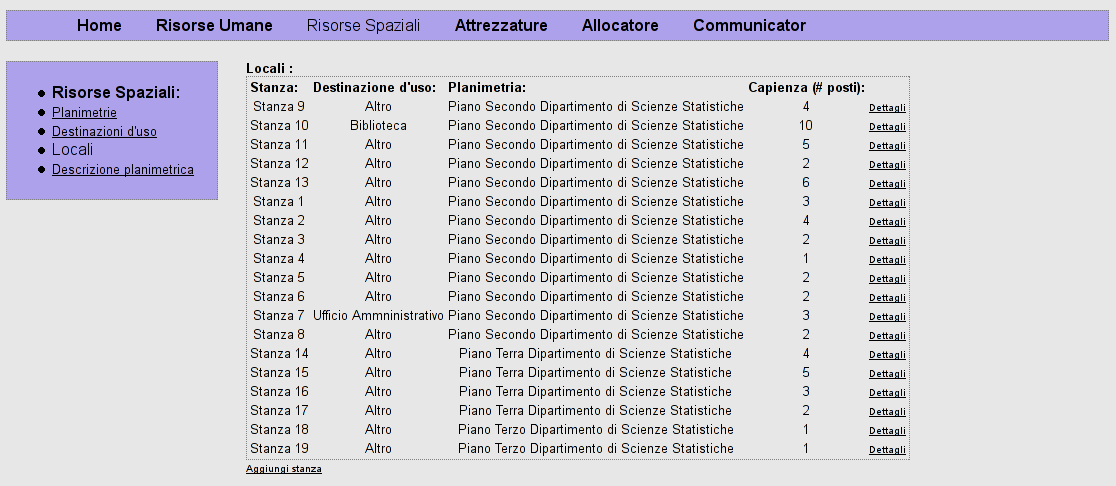
\includegraphics[width=5cm]{image/sres.png}
\caption {Componente di gestione delle risorse spaziali}
\label{sres}
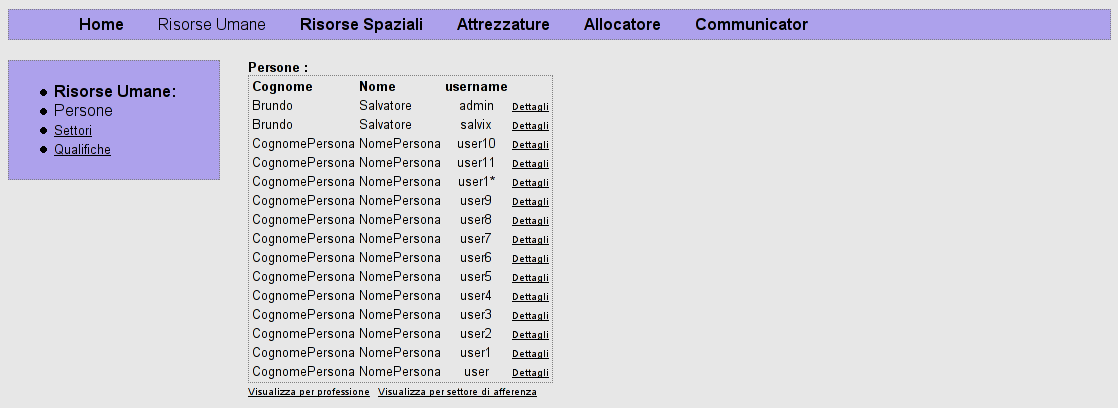
\includegraphics[width=5cm]{image/hres.png}
\caption {\emph{Tool} di controllo delle risorse umane}
\label{hres}
\label{alloc}
\end{figure}
\end{column}

\begin{column}{6cm}
\begin{figure}[htbp]
%\centering
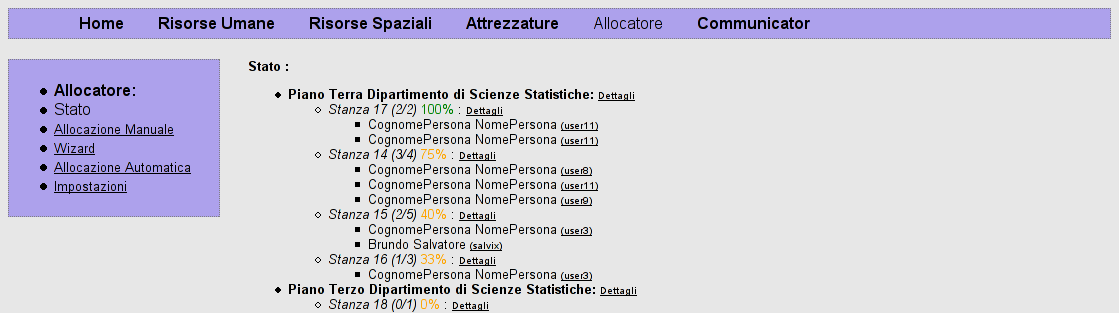
\includegraphics[width=5cm]{image/alloc.png}
\caption {Informazioni fornite dall'allocatore}
\label{sres}
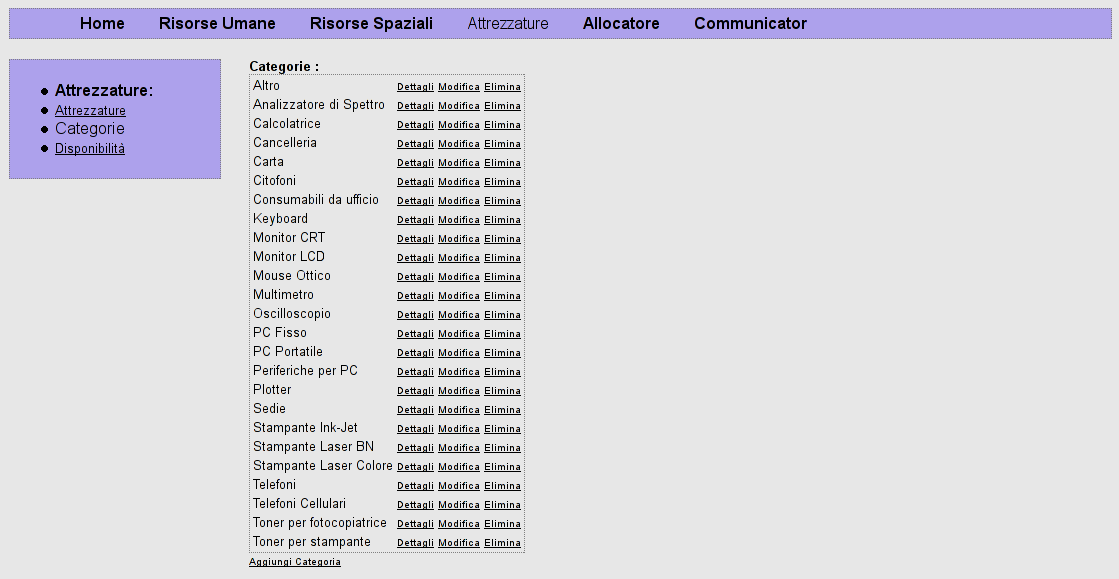
\includegraphics[width=5cm]{image/attr.png}
\caption {\emph{Tool} per la gestione delle attrezzature}
\label{hres}
\label{alloc}
\end{figure}
\end{column}

\end{columns}

\end{frame}



\begin{frame}
\frametitle{Conclusioni e sviluppi futuri}
\begin{block}{Sviluppi futuri}
\begin{itemize}
\item Modulo per l'allocazione automatica
\item Miglioramento dell'interfaccia mediante
l'utilizzo di soluzioni \emph{drag\&drop} via Javascript\cpr
\end{itemize}
\end{block}
\begin{block}{Conclusioni}
\begin{itemize}
\item Gli obbiettivi fondamentali
del lavoro si ritengono raggiunti
\item La modellizzazione della realtà è risultata apprezzabile
\item La struttura della \emph{Web-Application} è molto solida
\end{itemize}
\end{block}
\end{frame}


